\subsection{Localized evidence changes answers beyond generic image damage}
\label{sec:main-regional}

Figure~\ref{fig:behavior-region-specificity} tests the first level using the complete-answer sequence score. In the expanded 61-example set, Qwen and LLaVA have intervals above zero and Gemma's interval crosses zero; all three intervals lie above zero in the independently selected 52-example set. The first-token rank intervals are above zero for all six model-by-set comparisons (Appendix~\ref{app:detailed-results}). Together, these scores show that the annotated region contributes answer support beyond generic equal-area image damage in this compact-evidence setting.

\begin{figure}[!htbp]
    \centering
    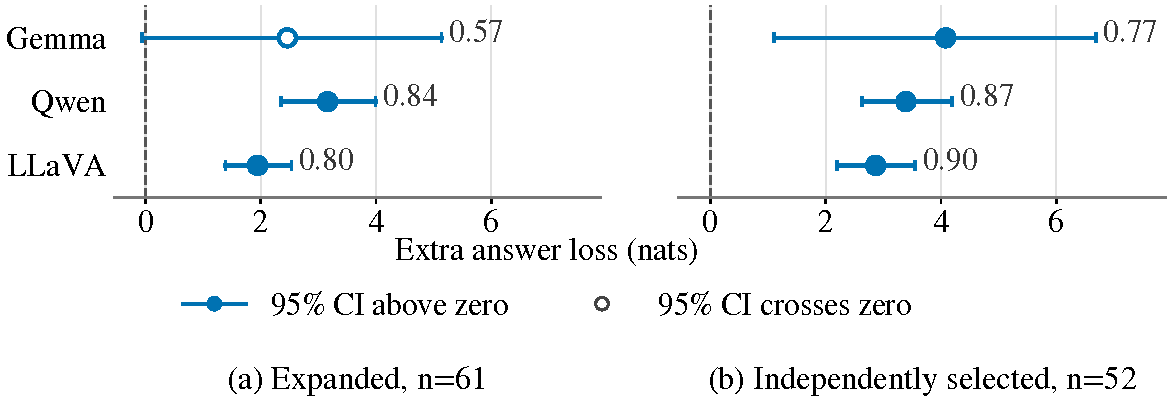
\includegraphics[width=\linewidth]{figures/2026-09-25-main-readable/behavior_region_specificity.pdf}
    \caption{\textbf{Answer-region corruption reduces complete-answer support beyond matched occlusion.} Panels (a) and (b) show separate sets of 61 and 52 compact-evidence examples on a shared raw log-probability scale. Each mark is the mean additional complete-answer score loss from masking the answer region rather than a same-area random region; whiskers are unadjusted 95\% sample-bootstrap intervals. Filled markers have intervals above zero; the hollow marker crosses zero. Numbers give positive-sample fractions. First-token rank results are in Appendix~\ref{app:detailed-results}.}
    \label{fig:behavior-region-specificity}
\end{figure}

\subsection{Clean hidden states recover the evidence-specific loss}
\label{sec:main-hidden}

Figure~\ref{fig:hidden-restoration-specificity} establishes the second level using the raw target-logit score: aligned clean hidden states recover more under answer-region corruption than under same-area random corruption. Gemma and Qwen show positive intervals across pooled visual positions, while LLaVA shows a positive interval at predefined answer-adjacent positions rather than across all visual positions. The first-token rank contrasts support the same position pattern (Table~\ref{tab:main-hidden-rank}). The independently selected 52-example grid retains this pattern. A separate 240-image evaluation freezes answer-position layers on 60 development images, then compares correct restoration with equal-norm random directions, reversed differences, and wrong insertion positions. All 12 jointly corrected differences are positive for the aligned restoration relative to their baselines or controls, connecting the regional score loss to specific internal content, direction, and location (Appendix~\ref{app:detailed-results}).

\par\smallskip
\noindent
\begin{minipage}{\linewidth}
    \captionsetup{type=figure,hypcap=false}
    \centering
    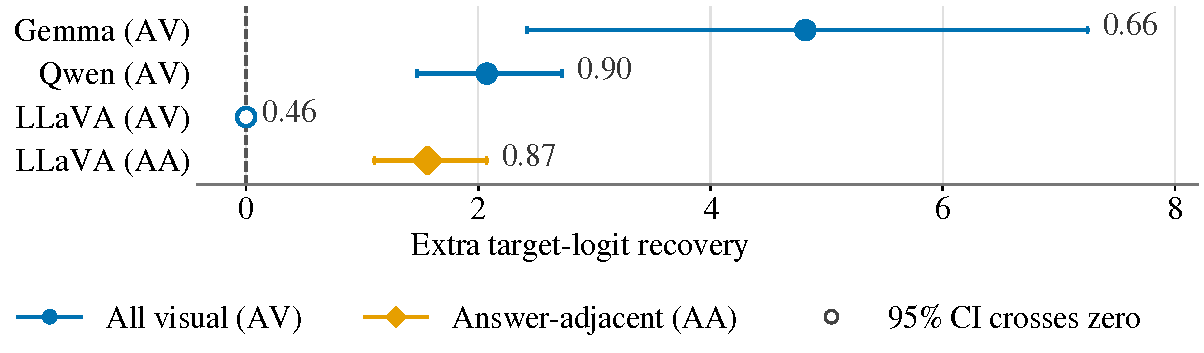
\includegraphics[width=\linewidth]{figures/2026-09-25-main-readable/hidden_restoration.pdf}
    \caption{\textbf{Aligned hidden restoration recovers additional target-logit support under evidence masking.} Raw answer-region-minus-random restoration effects on 61 examples; whiskers are unadjusted 95\% sample-bootstrap intervals. Filled marks lie above zero, the hollow mark crosses zero, and numbers give positive-sample fractions. AV pools visual positions; AA uses four answer-adjacent positions. Rank contrasts appear in Table~\ref{tab:main-hidden-rank}.}
    \label{fig:hidden-restoration-specificity}
\end{minipage}
\par\smallskip

\begin{minipage}{\linewidth}
    \captionsetup{type=table,hypcap=false}
    \caption{\textbf{Rank recovery follows the logit position pattern.} $\Delta s_{\mathrm{rank}}$ is the answer-mask restoration gain minus the same-area-random-mask gain on 61 examples. Brackets are unadjusted 95\% sample-bootstrap intervals; AV pools visual positions, and AA uses four answer-adjacent positions.}
    \label{tab:main-hidden-rank}
    \centering
    \normalsize
    \begin{tabular*}{\linewidth}{@{\extracolsep{\fill}}lrrr@{}}
    \toprule
    Model--position & $\Delta s_{\mathrm{rank}}\uparrow$ & 95\% interval & Positive fraction \\
    \midrule
    Gemma (AV) & 14,444.7 & [7,248.8, 23,404.2] & .738 \\
    Qwen (AV) & 2,711.5 & [549.4, 6,147.1] & .869 \\
    LLaVA (AV) & 1.23 & [-.25, 2.96] & .393 \\
    LLaVA (AA) & 500.2 & [124.9, 1,017.9] & .836 \\
    \bottomrule
    \end{tabular*}
\end{minipage}

\subsection{Effect matching distinguishes internal descriptions}
\label{sec:main-effect-matching}

The third level compares each candidate's two score effects with the complete intervention at its own interface. We first test compact fitted, native-channel, and shared-subspace descriptions, then use a frozen complete hidden state as a positive reference.

\subsubsection{Readable structure does not guarantee effect matching}
\label{sec:main-restricted}

The sparse comparison begins with reconstruction fidelity. On a separate 60-image development set (59 valid images for LLaVA), at 128 selected features the fitted tools have mean relative squared reconstruction errors (residual squared norm divided by full-change squared norm) of 1.76, 1.87, and 1.62 for Gemma, Qwen, and LLaVA, with mean direction similarities of .23, .22, and .20. Each error exceeds one: the squared reconstruction residual is larger than the squared complete change. The fitted tools therefore poorly reconstruct the internal change they are asked to explain (definitions in Appendix~\ref{app:detailed-setup}; per-model counts in Appendix~\ref{app:detailed-results}).

At matched feed-forward outputs on the same 240 evaluation images per model, Figure~\ref{fig:sparse-component-effects} shows no positive effect from the selected sparse reconstruction after correction over 72 tests. Yet the fitted tools' normalized feature summaries differ in 16 of 24 paired comparisons (Appendix Table~\ref{tab:sparse-structure-summary}). Readable structural variation and faithful reconstruction of a controlled answer effect are therefore distinct findings.

\par\smallskip
\noindent
\begin{minipage}{\linewidth}
    \captionsetup{type=figure,hypcap=false}
    \centering
    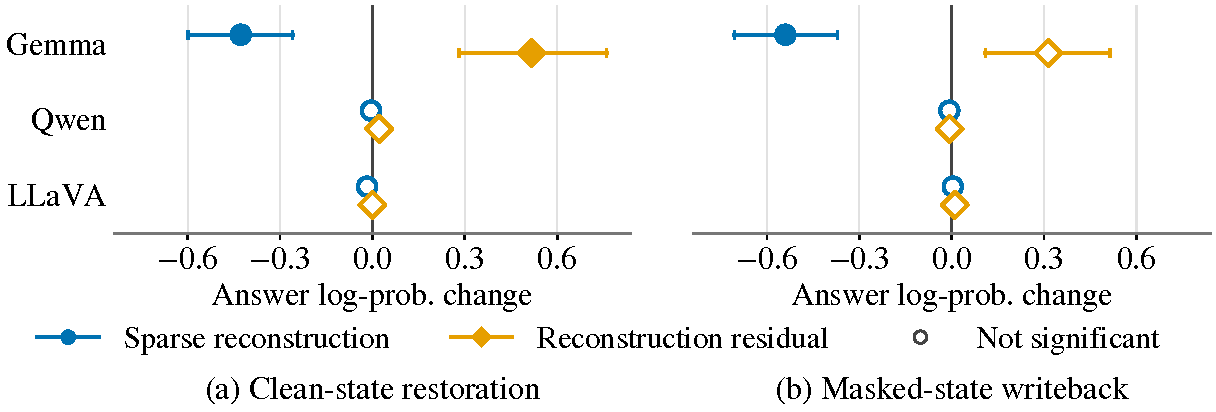
\includegraphics[width=\linewidth]{figures/2026-09-25-main-readable/sparse_component_effects.pdf}
    \caption{\textbf{Selected sparse reconstructions do not yield a reliable positive answer effect.} Panels (a) and (b) show restoration and masked-state writeback at the same feed-forward output on 240 images per model. Whiskers are uncorrected 95\% cluster-bootstrap intervals on a shared raw answer-score scale; filled marks survive the joint 72-test correction. Zero marks no score change.}
    \label{fig:sparse-component-effects}
\end{minipage}
\par\smallskip

Native feed-forward channels remove the fitted-tool reconstruction error and reveal local upstream--downstream links in all three models under positive-only selection. Their score effects, however, over-amplify the full-channel reference: Gemma's selected-group restoration changes the sequence score by 16.47, versus 3.79 for all channels (Appendix Table~\ref{tab:native-channel-path}). The two frozen channel rules select separately for each image using its known answer, and neither meets the full set of effect-matching criteria.

An example-shared linear subspace offers a different compact description. Figure~\ref{fig:main-low-rank-sweep} shows the eight candidate ranks on the 20-image selection set: no rank from 1 to 128 enters the effect-matching band in both directions. Table~\ref{tab:main-rank128} then reports diagnostic rank-128 effects on a separate 40-image set. Retaining hidden-change energy is not sufficient to match the answer effect: restoration can overshoot while masked-state writeback reverses direction. Appendix~\ref{app:detailed-results} reports the full controls and matched late-answer test.

\begin{minipage}{\linewidth}
    \captionsetup{type=figure,hypcap=false}
    \centering
    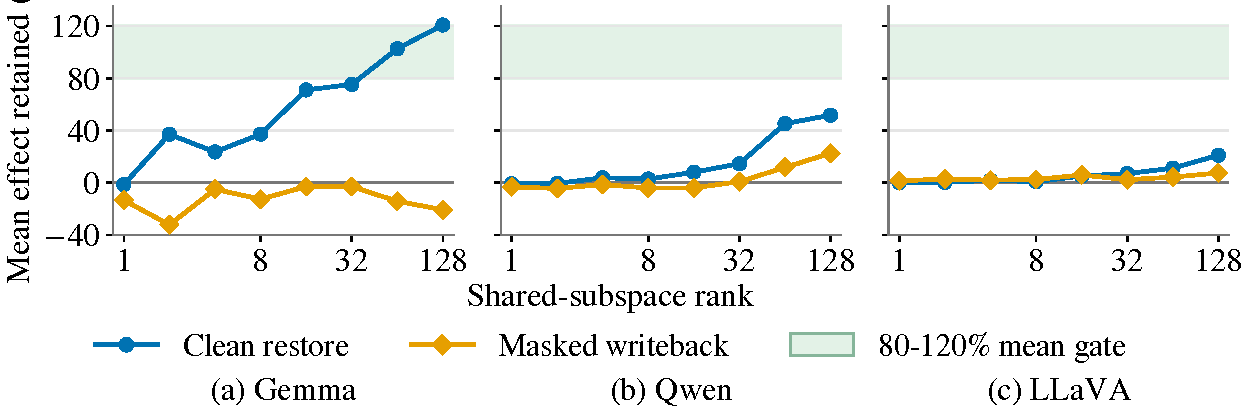
\includegraphics[width=\linewidth]{figures/2026-09-25-main-readable/low_rank_effect_matching.pdf}
    \caption{\textbf{No shared rank matches both directions.} Model-specific bases are fitted on 40 images; curves show restore/writeback effects for ranks 1--128 on a separate 20-image selection set, as percentages of mean natural clean-to-mask score change. Both must enter the shaded 80--120\% band at the same rank; none does.}
    \label{fig:main-low-rank-sweep}
\end{minipage}

\begin{minipage}{\linewidth}
    \captionsetup{type=table,hypcap=false}
    \caption{\textbf{Hidden-change energy does not ensure answer-effect matching.} Diagnostic rank-128 values on 40 separate images. Energy is retained squared hidden-change norm; restore/writeback are percentages of the mean natural score change. No rank passed selection.}
    \label{tab:main-rank128}
    \centering
    \normalsize
    \begin{tabular*}{\linewidth}{@{\extracolsep{\fill}}lrrr@{}}
    \toprule
    Model & Energy (\%) & Restore (\%) & Masked writeback (\%) \\
    \midrule
    Gemma & 88.9 & 425.0 & -357.7 \\
    Qwen & 53.1 & 53.0 & 51.2 \\
    LLaVA & 15.9 & 10.5 & 0.1 \\
    \bottomrule
    \end{tabular*}
\end{minipage}

\subsubsection{A complete LLaVA hidden state matches both directions}
\label{sec:main-full-hidden}

The complete hidden state provides a positive reference for effect matching. At LLaVA layer 30 and four answer-adjacent positions, restoration and masked-state writeback retain 93.0\% and 91.0\% of the mean clean-to-mask score change on the 20-image selection set, then 94.9\% and 92.4\% on a separate 40-image replication set. We freeze that interface before testing 60 accepted evidence masks reviewed without model results. On this independent set, clean-state restoration recovers 95.8\% and masked-state writeback removes 95.0\% of the mean natural clean-to-mask sequence-score change. All four predeclared paired-bootstrap bounds pass (Appendix Table~\ref{tab:llava-hidden-confirmation}); a post-hoc 15--30\% tolerance check gives the same decision (Appendix~\ref{app:gate-tolerance}). The same frozen internal location therefore nearly reproduces the natural score change in both directions.

A later same-sample comparison tests the penultimate language layer and four answer-adjacent positions in all three models. For LLaVA, this rule reuses the confirmed layer and positions under a common three-model run rather than selecting a new interface. At these matched relative locations, LLaVA again passes all four bounds (95.2\% restoration; 95.7\% writeback), Qwen reaches 74.3\% and 45.3\%, and Gemma's mean effects reverse direction. This common-location rule was chosen after the LLaVA confirmation, making the three-model comparison a diagnostic of the specified interfaces. Figure~\ref{fig:bidirectional-full-hidden} places it beside the independently confirmed LLaVA result; Appendix~\ref{app:detailed-results} reports its gate margins and sample-level accounting.

\par\smallskip
\noindent
\begin{minipage}{\linewidth}
    \captionsetup{type=figure,hypcap=false}
    \centering
    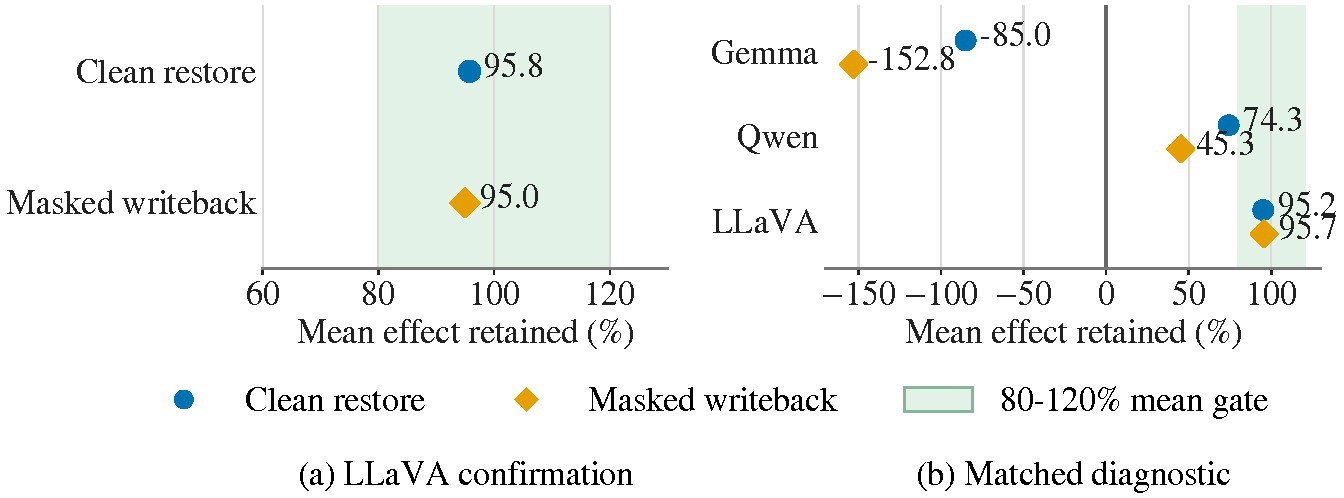
\includegraphics[width=\linewidth]{figures/2026-09-25-main-readable/full_hidden_bidirectional.pdf}
    \caption{\textbf{One independently confirmed complete hidden-state interface; a separate matched diagnostic.} Each mark divides the within-model mean restoration or masked-state-writeback effect by the mean clean-minus-masked sequence-score change. The shaded 80--120\% band is a mean gate, not a confidence interval. Panel (a) confirms the frozen LLaVA interface on 60 accepted masks with all four paired-bootstrap bounds passing. Panel (b) reuses those masks under a relative-layer rule chosen afterward; only the evaluated LLaVA interface passes all four bounds. Negative ratios reverse the mean effect; the panels use independent horizontal scales.}
    \label{fig:bidirectional-full-hidden}
\end{minipage}
\par\smallskip

\FloatBarrier
